\documentclass[showpacs, oneside, onecolumn, prl, amsmath, amssymb, nofootinbib, superscriptaddress, notitlepage]{revtex4-1}


\usepackage{cases}
\usepackage{amsmath}
\usepackage{amssymb}
\usepackage{amsfonts}
\usepackage{amssymb}
\usepackage{dcolumn}
\usepackage{bm}
\usepackage{bbm}
\usepackage{graphicx}
\usepackage{xcolor}
\usepackage{array}
\usepackage{subfigure}
\usepackage{hyperref}
\usepackage{multirow}

%%%%%%%%%%%%%%%%%%%%%%%%%%%%%%%%%%%%%%%%%%%%%%%%%%%%%%%%%%%%%%%%%%%%%%%%%%%%%%%%%%%
\newcommand{\bra}[1]{\langle #1\vert}
\newcommand{\ket}[1]{\vert #1\rangle}
\newcommand{\nn}{\nonumber \\}
\newcommand{\lag}{\langle}
\newcommand{\rag}{\rangle}
\newcommand{\cN}{{\cal N}}
\newcommand{\cA}{{\cal A}}
\newcommand{\gsim}{\mathrel{\hbox{\rlap{\lower.55ex \hbox {$\sim$}}
                   \kern-.3em \raise.4ex \hbox{$>$}}}}
\newcommand{\lsim}{\mathrel{\hbox{\rlap{\lower.55ex \hbox {$\sim$}}
                   \kern-.3em \raise.4ex \hbox{$<$}}}}

\newcommand\be{\begin{equation}}
\newcommand\ba{\begin{align}}
\newcommand\bas{\begin{align*}}
\newcommand\bt{\begin{table}}
\newcommand\bts{\begin{table*}}
\newcommand\bfig{\begin{figure}}
\newcommand\bfs{\begin{figure*}}
\newcommand\ee{\end{equation}}
\newcommand\ea{\end{align}}
\newcommand\et{\end{table}}
\newcommand\ets{\end{table*}}
\newcommand\efig{\end{figure}}
\newcommand\efs{\end{figure*}}
\newcommand\RA{$\ \ \Rightarrow\ \ $}


\newcommand\blue{\textcolor{blue}}
\newcommand\gray{\textcolor{gray}}
\newcommand\red{\textcolor{red}}




\hypersetup{colorlinks=true,
            breaklinks=true,
            pdfstartview=Fit,
            linkcolor=blue,
            citecolor=green,
            urlcolor=blue}

\bibliographystyle{apsrev4-1}




%%%%%%%%%%%%%%%%%%%%%%%%%%%%%%%%%%%%%%%%%%%%%%%%%%%%%%%%%%%%%%%%%%%%%%%%%%%%%%%%%%%
\begin{document}
	
\title{Problem set 4}


\author{JIAO Hao}


%%%%%%%%%%%%%%%%%%%%%%%%%%%%%%%%%%%%%%%%%%%%%%%%%%%%%%%%%%%%%%%%%%%%%%%%%%%%%%%%%%%
%\begin{abstract}
%
%\blue{Blue words are used to highlight mt questions.}
%
%\gray{Gray words show something I think by myself when reading these reviews, and I am not sure whather they are right.}
%
%\end{abstract}
%%%%%%%%%%%%%%%%%%%%%%%%%%%%%%%%%%%%%%%%%%%%%%%%%%%%%%%%%%%%%%%%%%%%%%%%%%%%%%%%%%%


\maketitle


%%%%%%%%%%%%%%%%%%%%%%%%%%%%%%%%%%%%%%%%%%%%%%%%%%%%%%%%%%%%%%%%
\subsection{Problem 1}

For an array f(x) with N point (x=0,1,...,N-1)

Make a Fourier transition of f(x):
\ba
&F(k)=\sum_{x=0}^{N-1}e^{-2\pi ik\cdot x}f(x)\\
\Rightarrow\ \ &f(x)=\sum_{k=0}^{N-1}e^{2\pi ik\cdot x}F(k)
\end{align}

And the Fourier transiform of a shift of this array f(x+y) is
\bas
F_y(k)&= \sum_{x=0}^{N-1}e^{-2\pi ik\cdot x/N}f(x+y)\\
&= \sum_{x=0}^{N-1}e^{-2\pi ik\cdot (x'-y)/N}f(x')\\
&= \sum_{x=0}^{N-1}e^{-2\pi ik\cdot x'/N}f(x')\times e^{2\pi ik\cdot y/N}\\
&= F(k)\times G_y(k)
\end{align*}
\bas
f(x-y)=ift[F_y(k)]=ift[dft[f(x)]\times G_y(k)]=[f\otimes g_y](x),
\end{align*}
where $g_y(x)=ift[G_y(k)]=\sum_{x=0}^{N-1}e^{-2\pi ik\cdot x/N}G_y(k)=\sum_{x=0}^{N-1}e^{-2\pi ik\cdot x/N}e^{2\pi ik\cdot y/N}$

\bfig
	\centering
	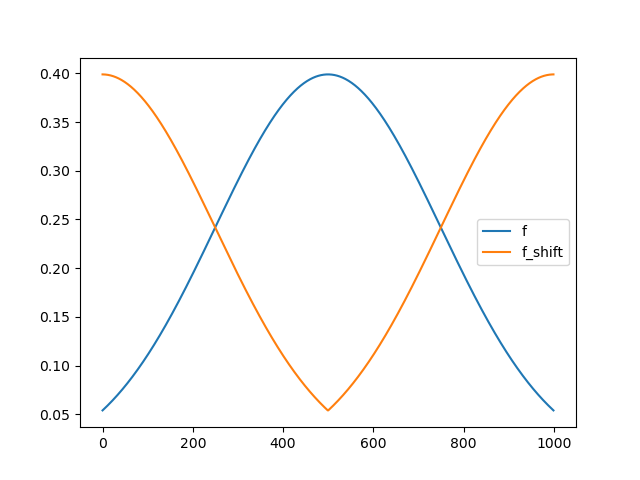
\includegraphics[scale=1]{4-1.png}
	\caption{Plot a gaussian that started in the centre of the array shifted by half the array length.}
	\label{4-1}
\efig

Plot a gaussian that started in the centre of the array shifted by half the array length in fig.\ref{4-1}

~~~~

%%%%%%%%%%%%%%%%%%%%%%%%%%%%%%%%%%%%%%%%%%%%%%%%%%%%%%%%%%%%%%%%
\subsection{Problem 2}

Make a Fourier transition of f(x) and g(y):
\ba
&F(k)=\sum_{x=0}^{N-1}e^{-2\pi ik\cdot x}f(x)\ \ ,\ \ f(x)=\sum_{k=0}^{N-1}e^{2\pi ik\cdot x}F(k)\\
&G(k)=\sum_{y=0}^{N-1}e^{-2\pi ik\cdot y}g(y)\ \ ,\ \ g(y)=\sum_{k=0}^{N-1}e^{2\pi ik\cdot y}G(k)
\end{align}

\bas
f*g(y)&=\int f(x)g(x+y)dx\\
&=\int dx\,\sum_{k=0}^{N-1}e^{2\pi ik\cdot x}F(k)\sum_{k'=0}^{N-1}e^{2\pi ik'\cdot(x+y)}G(k')\\
&=\int dx\,\sum_{k,k'=0}^{N-1}e^{2\pi i(k+k')\cdot x}F(k)G(k')e^{2\pi ik'\cdot y}\\
&=\sum_{k,k'=0}^{N-1}\frac1N\delta(k+k')F(k)G(k')e^{2\pi ik'\cdot y}\\
&=\frac1N \sum_{k=0}^{N-1}F(k)G(-k)e^{-2\pi ik\cdot y}\\
&=\frac1N \sum_{k=0}^{N-1}F(k)G^*(k)e^{-2\pi ik\cdot y}\\
&=ift(F(k)G^*(k))(y)\\
&=ift(dft(f)*conj(dft(g)))
\end{align*}

\bfig
	\centering
	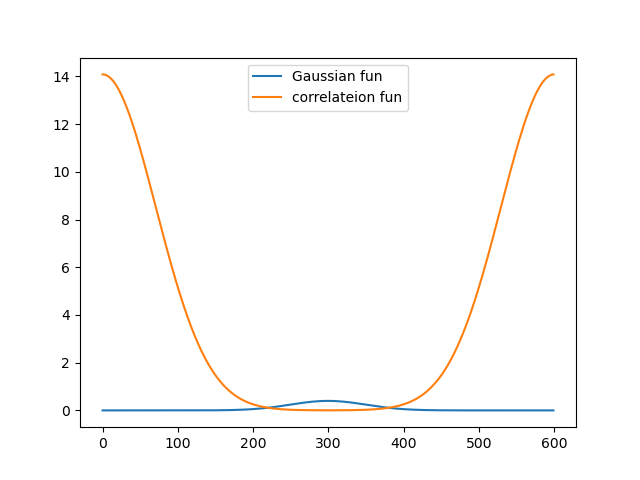
\includegraphics[scale=1]{4-2.png}
	\caption{Plot the correlation function of a Gaussian with itself.}
	\label{4-2}
\efig

Plot the correlation function of a Gaussian with itself in fig.\ref{4-2}

~~~~

%%%%%%%%%%%%%%%%%%%%%%%%%%%%%%%%%%%%%%%%%%%%%%%%%%%%%%%%%%%%%%%%
\subsection{Problem 3}

\bfig
	\centering
	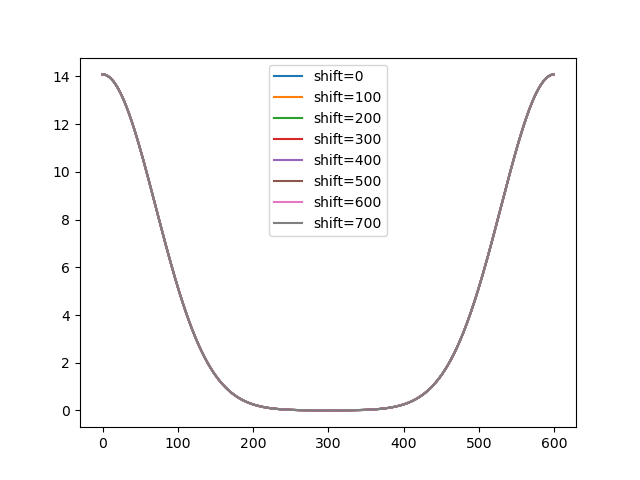
\includegraphics[scale=0.85]{4-3.png}
	\caption{Compare correlation function with different the shift.}
	\label{4-3}
\efig

\bfig
	\centering
	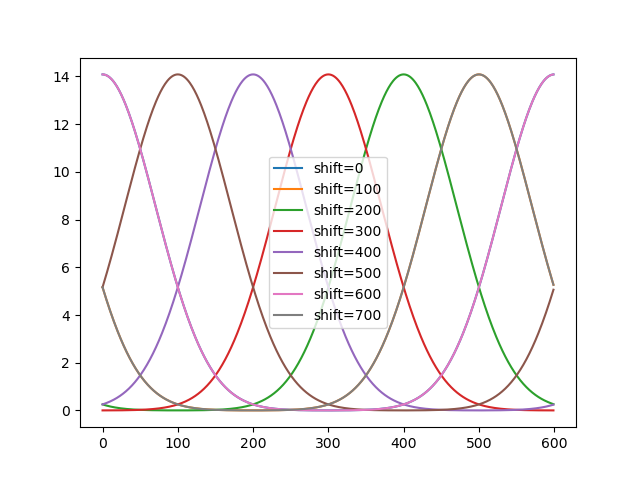
\includegraphics[scale=0.85]{4-3-2.png}
	\caption{Compare correlation function with different the shift (only shift 1 Gaussian).}
	\label{4-3-2}
\efig

I think here `take the correlation function of a Gaussian (shifted by an arbitrary amount) with itself': the itself is the shifted Gaussian function, is that right? If so, the result is shown in fig.\ref{4-3}. It is amazing that the shift does not affect at all.

If the `itself' means the unshifted Gausian function, the result is different: the the correlation function shift (shown in fig.\ref{4-3-2}).
 

~~~~

%%%%%%%%%%%%%%%%%%%%%%%%%%%%%%%%%%%%%%%%%%%%%%%%%%%%%%%%%%%%%%%%
\subsection{Problem 4}

\bfig
	\centering
	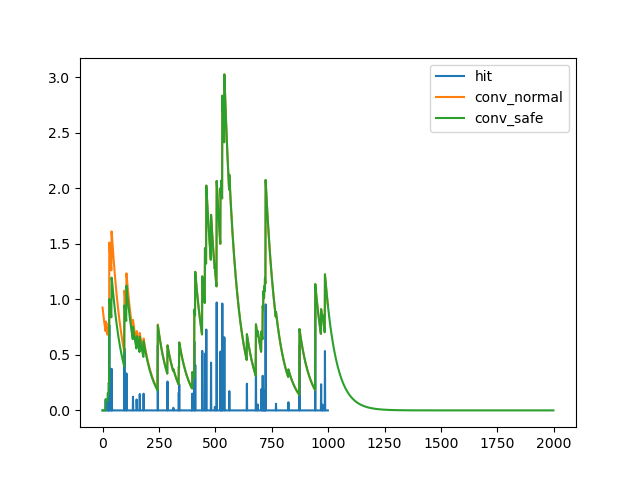
\includegraphics[scale=1]{4-4.png}
	\caption{Show the routine to take the convolution of two arrays without any danger of wrapping around. Take the example we show in the class}
	\label{4-4}
\efig

The result is show in fig.\ref{4-4}


~~~~

%%%%%%%%%%%%%%%%%%%%%%%%%%%%%%%%%%%%%%%%%%%%%%%%%%%%%%%%%%%%%%%%
\subsection{Problem 5}

\textbf{a) show that}
\be
\sum_{x=0}^{N-1}\exp(-2\pi ikx/N)=\frac{1-\exp(-2\pi ik)}{1-\exp(-2\pi ik/N)}
\ee

Set $\alpha=\exp(-2\pi ik/N)$. Then the lhs is
\bas
\sum_{x=0}^{N-1}\exp(-2\pi ikx/N)&=\sum_{x=0}^{N-1}\exp(-2\pi ik/N)^x=\sum_{x=0}^{N-1}\alpha^x\\
&=\frac{1-\alpha^N}{1-\alpha}=\frac{1-\exp(-2\pi ik)}{1-\exp(-2\pi ik/N)}
\end{align*}

$I=\sum_{x=0}^{N-1}\alpha^x$

$\alpha*I=\sum_{x=0}^{N-1}\alpha^{x+1}=\sum_{x=1}^N \alpha^{x}$

$I-\alpha I=(1-\alpha)I=\sum_{x=0}^{N-1} \alpha^{x}-\sum_{x=1}^N \alpha^{x}=1-\alpha^N$

$\Rightarrow\ \ I=(1-\alpha^N)/(1-\alpha)$ ,  if $\alpha\neq1$

\bfig
	\centering
	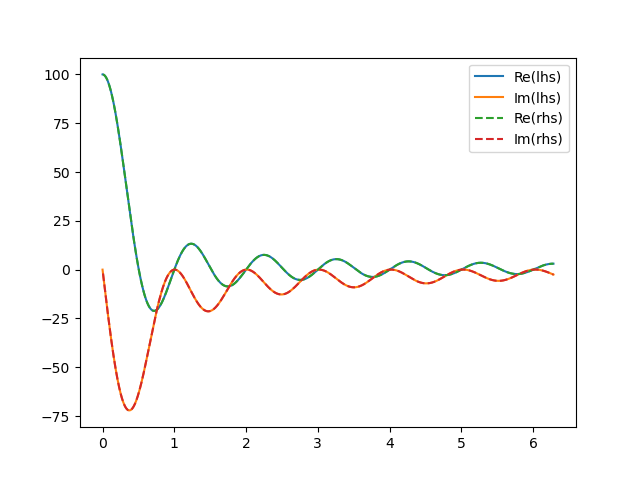
\includegraphics[scale=0.85]{4-5-1.png}
	\caption{Verify the result of Problem5 a).}
	\label{4-5-1}
\efig


~~~~

\textbf{b)} 

1. $k\rightarrow 0$: $\alpha=\exp(-2\pi ik/N)\rightarrow 1$. So the lhs$\rightarrow\sum_{x=0}^{N-1}1^x=N$

2. for any integer k that is not a multiple of N: This is the DFT of $f(x)\equiv 1$. As show in the class, the result is 0 except $k=nN,\ n\in\mathbb N$ (delta function).

~~~~

\textbf{c)} 

1. analytically write down the DFT of a non-integer sine wave.

\bas
DFT(\sin(2\pi k'x/N))&=\sum_{x=0}^{N-1}\sin(2\pi k'x/N)\exp(-2\pi ikx/N)\\
&=\sum_{x=0}^{N-1}\frac{e^{2\pi ik'x/N}-e^{2\pi ik'x/N}}{2i}\exp(-2\pi ikx/N)\\
&=\sum_{x=0}^{N-1}\frac1{2i}[\exp(-2\pi i(kx-k'x)/N)-\exp(-2\pi i(kx+k'x)/N)]\\
&=\frac1{2i}\left[\sum_{x=0}^{N-1}\exp(-2\pi i(k-k')x/N)-\sum_{x=0}^{N-1}\exp(-2\pi i(k+k')x/N)\right]\\
&=\frac1{2i}\left[\frac{1-\exp(-2\pi i(k-k'))}{1-\exp(-2\pi i(k-k')/N)}-\frac{1-\exp(-2\pi i(k+k'))}{1-\exp(-2\pi i(k+k')/N)}\right]
\end{align*}

\bfig
	\centering
	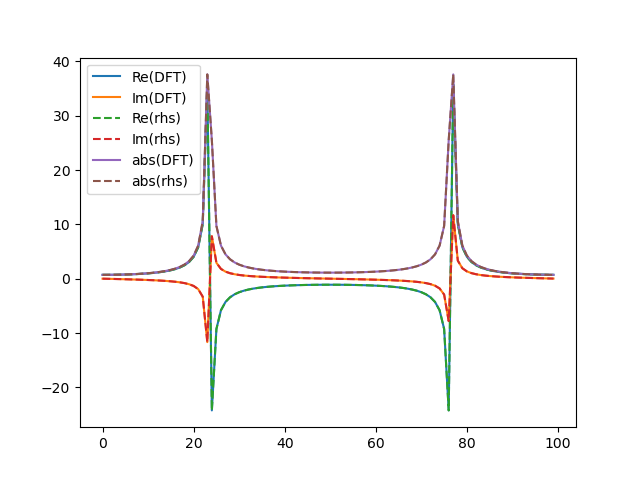
\includegraphics[scale=0.85]{4-5-3.png}
	\caption{The my analytic estimate of the DFT to the real one of a non-integer sine wave (The two are identical). Here I set k'=23.4.}
	\label{4-5-3}
\efig

Here I set $k'=23.4$ and the plot is show in fig.\ref{4-5-3}. To some degree, this result is similar to fat delta function at $k\sim k'\ or N-k',\ n\in \mathbb N$, but the peak are broaden and the DFT is non-zero even far away the peak.

\textbf{d) Show that when we multiply by this window, the spectral leakage for a non-integer period sine wave drops dramatically.}

\bfig
	\centering
	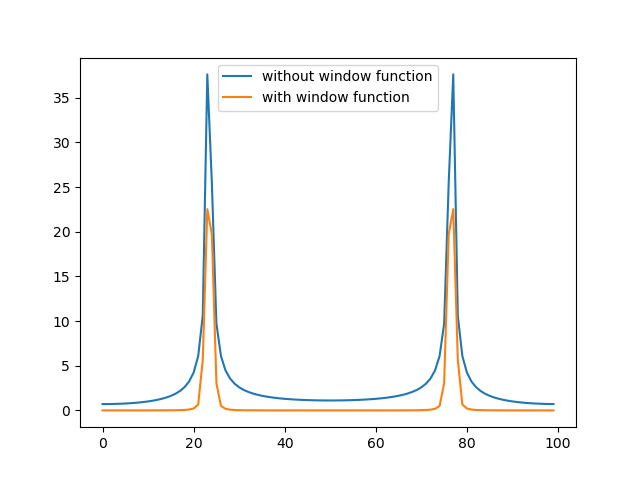
\includegraphics[scale=0.85]{4-5-4.png}
	\caption{Compare the DFT with and without window function. k'=23.4.}
	\label{4-5-4}
\efig

The result is show in fig.\ref{4-5-4}. It is real that the window function can cause the peak drops dramatically to 0. But the price is that the shape of peak changes.

~~~~

\textbf{e)}

\bfig
	\centering
	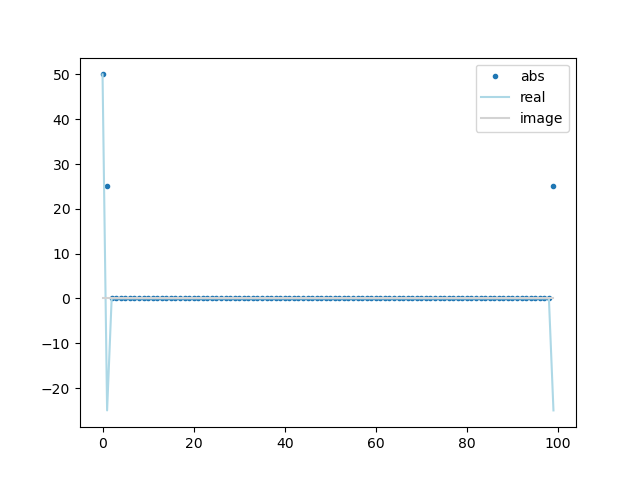
\includegraphics[scale=0.85]{4-5-5-1.png}
	\caption{Fourier transform of the window function. N=100.}
	\label{4-5-5-1}
\efig

1. Fourier transform of the window: 
\bas
&\,DFT[0.5-0.5\cos(2\pi x/N)](k)\\
=&\sum_{x=0}^{N-1}[0.5-0.5\cos(2\pi x/N)]\exp(-2\pi ikx/N)\\
=&\sum_{x=0}^{N-1}\left[0.5-\frac{e^{2\pi ix/N}+e^{2\pi ix/N}}{4}\right]\exp(-2\pi ikx/N)\\
=&0.5\sum_{x=0}^{N-1}\exp(-2\pi ikx/N)-\sum_{x=0}^{N-1}\frac14[\exp(-2\pi i(kx-x)/N)+\exp(-2\pi i(kx+x)/N)]\\
=&\frac12\frac{1-\exp(-2\pi ik)}{1-\exp(-2\pi ik/N)}-\frac1{4}\left[\frac{1-\exp(-2\pi i(k-1))}{1-\exp(-2\pi i(k-1)/N)}+\frac{1-\exp(-2\pi i(k+1))}{1-\exp(-2\pi i(k+1)/N)}\right]\\
=&\frac{1-A^{Nk}}{2-2A^{k}}-\frac14\left[\frac{1-A^{N(k-1)}}{1-A^{k-1}}+\frac{1-A^{N(k+1)}}{1-A^{k+1}}\right]
\end{align*}
where $A=\exp(-2\pi ix/N)$

The numerical result is show in fig.\ref{4-5-5-1}, here I set N=100. And I list the first and last four terms of the DFT: The error is approxmately 1e-15

- First four terms: [ 5.0000000e+01+0.00000000e+00j -2.5000000e+01+2.41473508e-15j
 -1.0904149e-16+1.31757938e-15j]

- Last four terms: [ 4.17403164e-16+1.24406761e-15j -1.51210335e-15-7.15809022e-16j
 -1.09041490e-16-1.31757938e-15j -2.50000000e+01-2.03250507e-15j]

So $W(k)\equiv\,$DFT(window)=[N/2, -N/4, 0,..., 0, -N/4]

~~~~

2. Get the windowed Fourier transform (denoted by $F_w(k)$) by appropriate combinations of each point in the unwindowed Fourier transform and its immediate neighbors:

The multiple in real space corresponds to convolution in Fourier space.
\bas
F_w(k)&=\frac1N\sum_{k'=0}^{N-1}W(k')F(k-k')\\
&=\frac1N\sum_{k'=-1}^1 W(k')F(k-k')\\
&=\frac1NW(-1)F(k-1)+W(0)F(k)+W(1)F(k+1)\\
&=-\frac14 F(k-1)+\frac12 F(k)-\frac14 F(k+1)
\end{align*}

$$\Rightarrow\ \ f_w(x)=IFT(F_w(k))(x)=IFT\left[-\frac N4 F(k-1)+\frac N2 F(k)-\frac N4 F(k+1)\right](x)$$

I compare the result with DFT of the windowed function in fig.\ref{4-5-5-2} so this expression is right.

\bfig
	\centering
	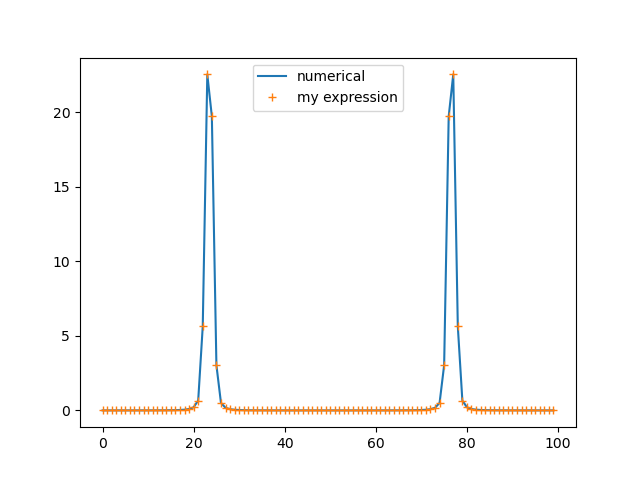
\includegraphics[scale=0.85]{4-5-5-2.png}
	\caption{Fourier transform of the window function. N=100.}
	\label{4-5-5-2}
\efig











\end{document}